\documentclass[../main.tex]{subfiles}

\begin{document}
	Die letzte in dieser Studienarbeit betrachtete Hardwarearchitektur ist die Grafikkarte (GPU). Moderne GPUs werden nicht nur zur Berechnung der auf dem Monitor gezeigten Inhalte genutzt, sondern können aufgrund ihrer Architektur auch für komplexe mathematische bzw. numerische Berechnungen genutzt werden. Die Vorzüge der Grafikkarte als Hilfsmittel zur Implementierung eines CNN und allgemein für aufwändige Rechenoperationen soll Abschnitt \ref{sec:cuda_berechnung} dieses Kapitels erläutert werden. Außerdem soll die Programmierung der Rechenoperationen auf GPUs am Beispiel von NVIDIAs CUDA-Umgebung gezeigt werden. Die Abschnitte \ref{sec:cuda_titan} \nameref{sec:cuda_titan} und \ref{sec:cuda_umsetzung} \nameref{sec:cuda_umsetzung} zeigen dann die in dieser Arbeit genutzte Hardware sowie den verfolgten Implementierungsansatz für ein Convolutional Neural Network. Leider konnte die Implementierung eines funktionsfähigen und lernenden CNNs auf CUDA nicht in der vorgegebenen Zeit beendet werden. Das entstandene System ist nicht in der Lage, die Muster des MNIST-Datensatzes korrekt zu klassifizieren. Der Fehler muss dabei in der Implementierung liegen, da das verwendete Netz in anderen Implementierungen ihren Zweck erfüllt und gute Ergebnisse in der Klassifizierung erzielt.
\section{Grafikkarten zur Berechnung} \label{sec:cuda_berechnung}
Der ursprüngliche Zweck von Grafikkarten war die Shader-Berechnung und damit waren GPUs ein dediziertes Werkzeug zur Berechnung der auf dem Bildschirm dargestellten Inhalte. Da aufwändige grafische Darstellungen auch viele Berechnungen für die steigende Zahl an Pixel bedeuten, haben sich Grafikkarten zu hochparallelen Recheneinheiten entwickelt. Ihre Möglichkeiten sind dabei im Vergleich zu general-purpose CPUs eingeschränkt, jedoch sind sie auf komplexe Matrixoperationen im \emph{floating point} -Format ausgelegt. Dabei besitzen sie eine Vielzahl an Rechenkernen, womit es möglich wird, eine große Masse an mathematischen Operationen parallel zu bearbeiten. \par Dieser Abschnitt beschäftigt sich mit der Programmierung von mathematischen Anwendungen auf Grafikkarten, im speziellen mit der CUDA-Programmierung und weist im Punkt \ref{sec:cuda_cublas} auf eine hilfreiche, von NVIDIA bereitgestellte Bibliothek hin. \par 
\subsection{Stärken und Schwächen der Grafikkarte} \label{sec:cuda_staerken}
Wie bereits erwähnt, sind moderne Grafikkarten in der Lage komplexe mathematische Operationen äußerst effizient durchzuführen, da sie über eine hohe Zahl an Recheneinheiten verfügen. Aktuelle Hochleistungs-Grafikkarte besitzen mehrere Tausend Rechenwerke. Im Fall von NVIDIAs CUDA werden diese \emph{CUDA-Cores} genannt. Der offensichtliche Vorteil der Verwendung von Grafikkarten für aufwändige Berechnungen liegt in der gegebenen hohen Parallelität (vgl. \cite{NVIDIA_HOMEPAGE}). GPUs verfügen dabei aber nicht über den Instruktionsumfang gängiger CPUs. Generell kann festgestellt werden, das GPUs nicht für komplex verschachtelte Programmabläufe geeignet sind. Sie sind auf Rechenoperationen spezialisiert und eignen sich nur bedingt für andere Programmabläufe. Speziell besitzen Grafikkarten nur bedingte Möglichkeiten zur \emph{branch prediction} (Verzweigungsvorhersage). \par Außerdem benötigen GPUs immer eine CPU, die Rechenoperationen oder Programme auf der Grafikkarte startet und diese kontrolliert und koordiniert. Ein weiterer entscheidender Nachteil von modernen leistungsstarken Grafikkarten ist ihr hoher Preis. Im Vergleich zu hochwertigen CPUs sind Grafikkarten sehr teuer. Der Einsatz von GPUs für mathematische Berechnungen ist daher nur sinnvoll, wenn eine hohe Zahl an Rechenoperationen notwendig ist oder eine große Datenmenge im Sinne von Berechnungen verarbeitet werden muss. Das Problem muss sich dabei auch geeignet parallelisieren lassen, da sonst der Vorteil der Grafikkarte erlischt. \par Der nächste Abschnitt \ref{sec:cuda_unterschiede} soll die allgemeine Architektur einer modernen NVIDIA CUDA-fähigen Grafikkarte darstellen und damit den hier erwähnten Vorteil der Parallelität unterstreichen. \par 
\subsection{Architektur moderner Grafikkarten} \label{sec:cuda_unterschiede}
Prinzipiell sind die Architekturen der aktuellen NVIDIA Grafikkarten gleich aufgebaut. Eine Grafikkarte besteht dabei aus \emph{Streaming Multiprocessors (SM)}, den CUDA-Cores, einem dedizierten Graphikspeicher mit entsprechenden Caches und Speicher-Controllern. \par 
\begin{figure}[!htbp]
	\centering
	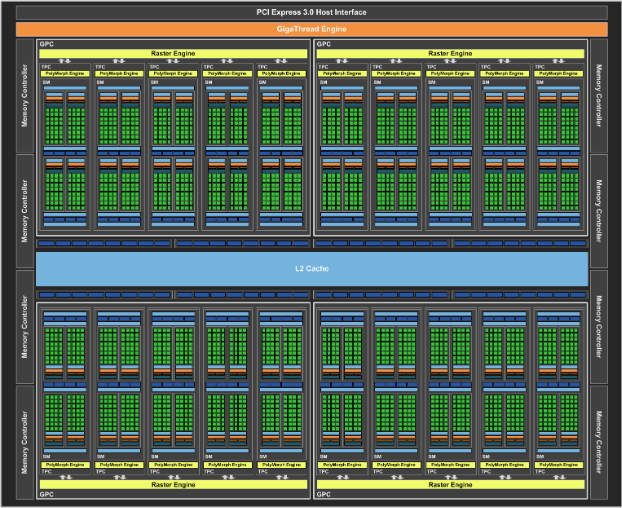
\includegraphics[width=0.8\linewidth]{../images/Riedle/architektur_pascal_komplett.png}
	\caption{Grafikkartenarchitektur am Beispiel der Pascal-Architektur von NVIDIA ( \cite{Pascal_white})} \label{pic:cuda_pascal_compl}
\end{figure}
Abbildung \ref{pic:cuda_pascal_compl} zeigt die erwähnten Komponenten in ihrem Zusammenspiel am Beispiel der Pascal-Architektur von NVIDIA. Diese findet beispielsweise in Grafikkarten vom Typ GTX 1080 Ti Anwendung. Von oben beginnend, ist in Abbildung \ref{pic:cuda_pascal_compl} die PCIe-Schnittstelle zum Host-System gezeigt. Das Host-System bildet die bestimmende CPU. Darunter folgt die GigaThread-Engine. Weiter ist die GPU in GPCs (Graphic Processing Clusters) unterteilt. Diese besitzen je eine Raster Engine und greifen auf den selben L2-Cache zu (vgl. \cite{Pascal_white}). Die GPCs sind weiter unterteilt in je zehn SMs.  Die Streaming Multiprocessors teilen die Arbeit auf in dieser Architektur 128 CUDA-Cores auf. Jede SM besitzt dabei eine separaten L1-Cache. \par 
\begin{figure}[!htbp]
	\centering
	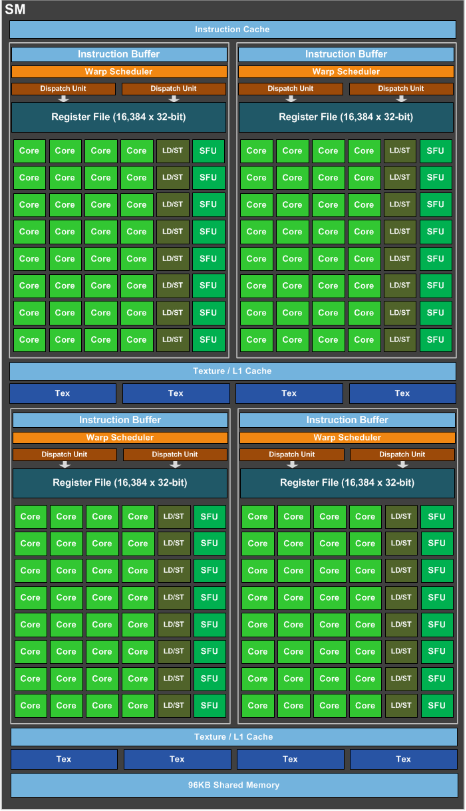
\includegraphics[width=0.8\linewidth]{../images/Riedle/architektur_pascal.png}
	\caption{Aufbau eines Streaming Multiprocessors in der Pascal-Architektur (\cite{Pascal_white})} \label{pic:cuda_sm}
\end{figure}
In Abbildung \ref{pic:cuda_sm} ist eine detaillierte Darstellung einer SM gegeben (vgl. \cite{Pascal_white}). Ein Streaming Multiprocessor besteht dabei aus vier Blöcken, auf die sich die 128 CUDA-Cores pro SM aufteilen. In der Abbildung sind zur besseren Übersicht weniger Cores aufgetragen. Jeder dieser Blöcke besitzt einen dedizierten \emph{Instruction Buffer}, einen \emph{Warp Scheduler} und ein sogenanntes \emph{Register File}. Darin sind 16384 32-Bit Register abgebildet. \par 
Ein Warp ist in CUDA eine Einheit von 32 Threads. Die CUDA-Struktur bildet alle erzeugten Threads in solche Warps ab und verteilt diese entsprechend innerhalb eines SM. Außerdem besitzt jede SM zwei L1-Caches und acht \emph{Texture Units}. Des weiteren besitzt jeder Streaming Multiprocessor einen dedizierten Shared-Memory-Bereich.\par 
Nachdem nun in diesem Abschnitt auf die grundlegende Architektur von NVIDIAs Grafikkarten am Beispiel der Pascal-Architektur eingegangen wurde, soll im Abschnitt \ref{sec:cuda_programmierung} auf einige Aspekte der CUDA-Bibliothek und damit der Programmierung von Anwendungen auf CUDA-fähigen Grafikkarten eingegangen werden. Die als Zielhardware für diesen Projektteil verwendete NVIDIA GTX Titan X Grafikkarte ist mit der sogenannten Maxwell Architektur ausgestattet. Diese wird in Abschnitt \ref{sec:cuda_titan} näher erläutert. \par 
\subsection{CUDA Programmierung} \label{sec:cuda_programmierung}
Die CUDA-Programmierung basiert auf der Programmierung von sogenannten \emph{Kernels}. Ein Kernel stellt dabei eine Routine dar, welche auf einer GPU ausgeführt werden kann. \par 
\begin{lstlisting}[language=C, caption=Minimaler Kernel, captionpos=b, label=listing:min_kernel]
	__global__ void minimal_kernel(float* a, float* b, float* c, 
									int size)
	{
		for(int i = 0; i < size; i++)
		{
			c[i] = a[i] + b[i];
		}		
	}
\end{lstlisting}
Listing \ref{listing:min_kernel} zeigt einen simplen CUDA-Kernel. Dieses Minimalbeispiel nimmt drei Zeiger auf \texttt{floats} und eine Ganzzahl als Parameter. Er addiert dabei einfach elementweise die Inhalte der Arrays \texttt{a} und \texttt{b} und speichert das Ergebnis im Array \texttt{c}. Im momentanen Zustand wird die \texttt{for} -Schleife seriell auf der GPU ausgeführt. Zur Parallelisierung später in diesem Abschnitt mehr. Wichtig ist hier der Specifier \texttt{\_\_global\_\_}. Er definiert einen CUDA-Kernel. Solche Kernels können nun vom Host aus auf der Grafikkarte gestartet werden (vgl. \cite{CUDA_GUIDE}). Der Host ist in jedem Fall die CPU und der darauf laufende Teil des Programmcodes. Mit dem Specifier \texttt{\_\_device\_\_} können Subroutinen auf der GPU deklariert werden. Solche Funktionen dürfen nur von Kernels auf der GPU aufgerufen werden. \\ Es ist zu beachten, dass die übergebenen Arrays \texttt{a}, \texttt{b} und \texttt{c} auf im Speicher der GPU liegen müssen. Die Grafikkarte hat keinen direkten Zugriff auf den RAM des Systems. Es muss also immer ein Transfer der Daten vom Host über die PCIe-Schnittstelle des Systems auf das Device (Grafikkarte) und zurück erfolgen. Dazu bietet die CUDA- Library spezielle Funktionen an. \par 
Bei der CUDA- Library handelt es sich um eine C/C++ -Bibliothek. Diese stellt verschiedene Funktionen zur Kommunikation und Kontrolle der GPU vom Host aus zur Verfügung. Wichtige Funktionen stellen dabei die Methoden \texttt{cudaMalloc(..)}, \texttt{cudaFree(..)} und \texttt{cudaMemcpy(..)} dar. Damit wird der Zugriff auf den Speicher der Grafikkarte vom Host aus geregelt. \par 
\begin{lstlisting}[language=C, caption=Aufruf des minimalen Kernels mit Speicherzugriff vom Host, captionpos=b, label=listing:min_kernel_host, breaklines]
	float *A_host, *B_host, *C_host;
	float *A_device, *B_device, *C_device;
	
	A_host = malloc(ARRAY_SIZE_D*sizeof(float));
	B_host = malloc(ARRAY_SIZE_D*sizeof(float));
	C_host = malloc(ARRAY_SIZE_D*sizeof(float));
	
	fillArrays(A_host, B_host, ARRAY_SIZE_D); /* Hilfsroutine um den Arrays Werte zuzuweisen */
	
	cudaStatus_t cuda_state;
	
	cuda_state = cudaMalloc((void**) &A_device, ARRAY_SIZE_D*sizeof(float));
	cuda_state = cudaMalloc((void**) &B_device, ARRAY_SIZE_D*sizeof(float));
	cuda_state = cudaMalloc((void**) &C_device, ARRAY_SIZE_D*sizeof(float));
	
	cuda_state = cudaMemcpy((void*) A_device, (void*) A_host, ARRAY_SIZE_D*sizeof(float), cudaMemcpyHostToDevice);
	cuda_state = cudaMemcpy((void*) B_device, (void*) B_host, ARRAY_SIZE_D*sizeof(float), cudaMemcpyHostToDevice);
						
	minimal_kernel<<<1,1>>>(A_device, B_device, C_device);
	
	cuda_state = cudaMemcpy((void*) C_host, (void*) C_device, ARRAY_SIZE_D*sizeof(float), cudaMemcpyHostToDevice);
	
	cuda_state = cudaFree((void*) A_device);
	cuda_state = cudaFree((void*) B_device);
	cuda_state = cudaFree((void*) C_device);
\end{lstlisting}

\subsection{cuBLAS (Basic Linear Algebra Sub-Routines)} \label{sec:cuda_cublas}
\section{Verwendete Hardware: GTX Titan X} \label{sec:cuda_titan}
\section{Umsetzung} \label{sec:cuda_umsetzung} 
\subsection{Unrolling-based Convolution} \label{sec:cuda_unrolling_conv}
\subsection{Input-Layer} \label{sec:cuda_input}
\subsection{Convolutional-Layer} \label{sec:cuda_conv}
\subsection{MaxPooling-Layer} \label{sec:cuda_pooling}

\end{document}